\documentclass[a4paper,12pt]{article}

\usepackage[utf8]{inputenc}
\usepackage{polski}
\usepackage{fullpage}
\usepackage{hyperref}
\usepackage[pdftex]{graphicx} % Wsparcie dla obrazkow
\usepackage{listings}
\usepackage{lscape}

\newtheorem{df}{Definicja}

\title{Wyznaczanie reprezentacji preferencji uniwersalnych}
\author{Bartosz Górski \and Marcin Kaczyński \and Paweł Sokołowski}

\begin{document}

\maketitle

\section{Opis zadania} 

Tematem zadania jest wyszukiwanie preferencji uniwersalnych.\\

Klasa Y jest preferowana wobec klasy $X$ wtedy i tylko wtedy gdy każdy obiekt należący do klasy $Y$ jest preferowany wobec każdego obiektu z klasy $X$. Definicję można wyrazić w następujący sposób: dla każdego obiektu z klasy $X$ istnieje obiekt z klasy $Y$ który jest względem niego preferowany.  \\

Dla rozważań na temat preferencji na poziomie atrybutów, a nie klas, należy również zdefiniować kontekst preferencji. Oznaczamy go jako:

			$$K = (G,M,I)$$

gdzie $G$ to zbiór obiektów, $M$ to zbiór atrybutów, a $I$ to relacja $G \times M$, która mówi nam, jakie obiekty ze zbioru $G$ posiadają jakie atrybuty ze zbioru $M$. \\

W tym kontekście możemy z kolei sformułować definicję preferencji uniwersalnych na poziomie atrybutów:

\begin{df}{}{}{
Zbiór atrybutów $B$ należący do $M$ jest uniwersalnie preferowany względem zbioru atrybutów $A$ należącego do $M$ wtedy i tylko wtedy gdy zbiór wszystkich obiektów $B'$ posiadających wszystkie atrybuty z $B$ jest preferowany względem zbioru wszystkich obiektów $A'$ posiadających wszystkie atrybuty z $A$. Można to także określić w taki sposób, że $B$ jest preferowane względem $A$ jeżeli $B'$ należy do zbioru klas lepszych od $A'$.}
\end{df}

Wobec powyższego celem zadania jest ustalenie, czy na podstawie wiedzy o preferencji klasy $Y$ wobec klasy $X$, możemy znaleźć preferencje różnych podzbiorów atrybutów klasy $Y$ wobec tych z klasy $X$. \\

Dla przykładu załóżmy, że każdy samochód można uznać za obiekt posiadający pewną liczbę atrybutów (marka, rok produkcji, cena, liczba drzwi, pojemność silnika itd.). Można je również zaklasyfikować do danej klasy samochodów, ze względu na kraj produkcji, typ auta, lub jakikolwiek inny atrybut. Badając preferencje uniwersalne, chcemy stwierdzić, czy fakt że osoba A woli samochody małe od dużych oznacza na przykład, że woli samochody o niskim spalaniu paliwa od tych o wysokim, czy też powód leży gdzieś indziej.

\section{Założenia}


Mając podstawowe definicje pojęć z tematyki naszych rozważań możemy przejśc do podstawowych założen. \\
\begin{itemize}
\item Mamy zdefiniowane relacje pomiędzy klasami, a nie obiektami należącymi do tych klas.
\item Algorytm pracuje na danych w postaci transakcyjnej.
\end{itemize}

\section{Dane wejściowe i wyjściowe}
\label{opis_danych}
Dane wejściowe są przekazywane do aplikacji w postaci następujących plików:
\begin{itemize}
\item plik zawierający zbiór danych
\item plik z opisem relacji
\end{itemize}
Obsługiwanym formatem plików zawierających zbiór danych jest Csv. Wymagane jest aby w jednej z kolumn przechowywane były dane określające do której klasy należy dany wiersz. Poniżej został przedstawiony przykładowy plik: \\

\begin{tabular}{l}
low,low,4,2,big,high,unacc \\
low,low,4,4,small,low,unacc \\
low,low,4,4,small,med,acc \\
low,low,4,4,small,high,good \\
\end{tabular}
\\

W kolejnych kolumnach znajdują się atrybuty określające pewne właściwości zbioru danych. Separatorem oddzielającym kolumny jest znak ','. W przykładowym pliku nazwa klasy do której przynależy znajdujący się w danym wierszu obiekt znajduje się w ostatniej kolumnie, nic nie stoi jednak na przeszkodzie, aby w ten sposób interpretować dane znajdujące się w innej kolumnie. \\

Kolejnym plikiem wejściowym aplikacji jest opis relacji pomiędzy klasami. Plik ten składa się z wielu linii. W każdej z nich znajduje się wpis typu:\\

\begin{tabular}{l}
a$<$b \\
\end{tabular} \\

\begin{figure}[h!]
\begin{center}
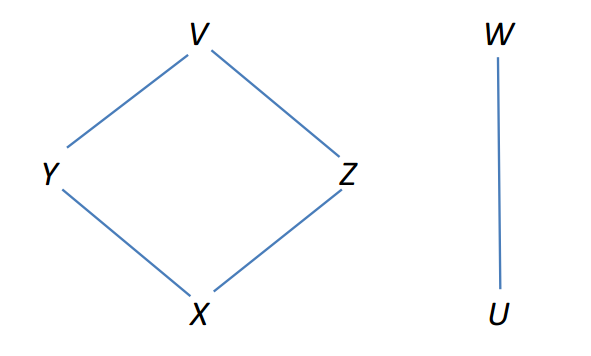
\includegraphics[width=0.5\textwidth]{img/relations.png}
\caption{Przykładowy graf relacji}
\label{relat2}
\end{center}
\end{figure}

Oznacza on, że klasa {\bf a} jest w relacji z klasą {\bf b}.
Dla przykładowego grafu relacji (\ref{relat2}) plik powinien być postaci: \\

\begin{tabular}{l}
Y$<$V \\
Z$<$V \\
X$<$Y \\
X$<$Z \\
U$<$W \\
\end{tabular}
\\

Dane wyjściowe wyświetlane są w polu tekstowym wewnątrz aplikacji. W każdej linii znajduje się opis jednego ze znalezionych minimalnych wzorców. Przykładowe wyjście programu: \\

\begin{tabular}{l}
1. (4\#other meal) =$>$ (3\#meal containing alcohol) \\
2. (2\#non-vegetarian meal without pork, 3\#meal containing alcohol) =$>$ () \\
3. (4\#other meal, 3\#meal containing alcohol) =$>$ () \\
\end{tabular}
\\

W nawiasach wymienione są opisy znalezionych atrybutów postaci: \{numer kolumny\}\#\{wartość atrybutu\}. Dane w lewym i prawym nawiasie przedstawiają atrybuty odpowiednio z lewego i prawego obiektu. 
\section{Szczegóły implementacji}

Implementacja została przygotowana w języku C\# i działa na platformie .NET Framework 4.0. Implementacja związana z algorytmem została podzielona na 4 projekty: Algorithm, DAL, HashTree i pomocniczy projekt Common.\\

W projekcie Algorithm znajdują się wszystkie klasy i interfejsy w bezpośredni sposób związane z interfejsem. Projekt DAL zawiera implementacje dostępu do danych, a więc w tym przypadku parsowanie plików z danymi do postaci wykorzystywanej w algorytmie. W projekcie HashTree znalajdują się interfejsy i implementacja drzewa mieszającego. Projekt Common zawiera wspólne klasy wykorzystywane w pozostałych projektach. W projekcie Common znajdują się niemal jedynie obiekty DTO. Obiekty te same w sobie nie wykonują operacji, dlatego nie będą szczegółowo opisywane.\\

W celu zapewnienia elastyczności skorzystano w projekcie ze wzorca Dependency Injection. Zgodnie z wzorcem, na implementację algorytmu składa się szereg interfejsów, których odpowiedzialności przedstawiaja się następująco:\\

Za główny interfejs można uznać \textit{IAlgorithm}, a jego podstawowym zadaniem jest znajdowanie preferencji uniwersalnych. Interfejs jest implementowany przez klasy \textit{Generators} i \textit{ModifiedApriori}. Podstawowa różnica pomiędzy klasami polega na tym, że klasa Generators do obliczania minimalnych preferencji wykorzystuje informację o generatorach do odrzucania większej liczby zbiorów kandydujących. Obie implementacje operują na wierszach
typu \textit{Row}/\textit{SimpleRow}, które są odwzorowaniem danych w postaci wygodnej do prowadzenia obliczeń. Do znajdywania zbiorów kandydujących wykorzystywany jest interfejs \textit{ICandidatesGenerator}. Za znajdowanie podzbiorów wspieranych w transakcjach odpowiada \textit{IHashTree}. Wczytywanie danych odbywa się za pomocą \textit{IDataManager}, a konwersja wyników do postaci wygodnej dla użytkownika za pomocą \textit{IResultsConverter}.\\

Ogólnie przebieg działania całego algorytmu składa się z następujących kroków:

\begin{enumerate}
\item wczytanie i parsowanie danych,
\item wykonanie obliczeń,
\item parsowanie wyników do czytelnej postaci
\end{enumerate}

Wykonanie obliczeń (2) przebiega wg następującego schematu:\\

W kolejnych iteracjach znajdywane są nowe zbiory kandydujące, dla wszystkich zbiorów obliczane są dwa liczniki mówiące o tym jakie wsparcie mają te zbiory w klasie transakcji spełniających i nie spełniających relację. Aby zapewnić wydajne obliczanie wartości omawianych liczników, wykorzystywane jest drzewo mieszające tworzone w każdej iteracji dla zbioru kandydatów. Po obliczeniu liczników podejmowana jest decyzja o tym, czy dany kandydat
jest minimalnym wzorcem, czy należy go odrzucić lub analizować dalej. Na tym etapie (opcjonalnie) podejmowana jest decyzja czy któryś z podzbiorów danego zbioru kandydującego jest generatorem. Jeżeli tak, taki zbiór nie będzie analizowany dalej.
\subsection{Generowanie kandydatów}
Poniższy pseudokod przedstawia algorytm generowania nowych kandydatów o długości $n+1$. \\
\begin{center}
\begin{lstlisting}[numbers=left]
List<ushort[]> GenerateCandidates(List<ushort[]> previous)
{
  tree = CreateTree(previous);
  foreach(left in previous)
  {
    right = left.next()
    while(right[1:n-1] = left[1:n-1])
    {
      new = buildNewCandidate(left, right)
      if(tree.checkSupport(new)
        results.add(new);
      right = right.next()
    }
  }
  return results;
}
\end{lstlisting}
\end{center}

W algorytmie założono, że transakcje znajdujące się w liście \textit{previous} są posortowane zgodnie z porządkiem słownikowym. Sposób ich generowania oraz pozostałe elementy algorytmu zapewnieją utrzymania tego porządku dla dłuższych transakcji.
W 3 linii algorytmu ze zbioru transakcji o długości $n$ budowane jest drzewo mieszające. Pozwala ono w efektywny sposób sprawdzać w linii 10 czy wszystkie podzbioru o długości $n$ transakcji \textit{new} są wspierane w zbiorze \textit{previous}. \\

Złożoność algorytmu w przypadku pesymistycznym jest równa $O(n^2)$. Jednak utrzymywanie posortowanej listy \textit{previous} pozwala na przerywanie pętli wewnętrznej (linia 7) w momencie gdy transakcje \textit{left} i \textit{right} różnią się chociażby na jednej z pierwszych $n-1$ pozycji. Pozwala to na znaczne ograniczenie spodziewanej złożoności algorytmu.
\subsection{Złożoność}
W tym rozdziale zostanie omówiona złożoność algorytmu. Zostały przyjęte następujące oznaczenia.
\begin{itemize}
\item $ n$ - liczba wejściowych transakcji
\item $ m$ - długość wejściowych transakcji
\item $ N = n^2$ - liczba transakcji powstałych po połączeniu transakcji w pary
\item $ M = 2m$ - długość transakcji po połączeniu transakcji w pary
\item $ L_i$ - liczba rozważanych transakcji w obrocie pętli algorytmu (linia 1) o numerze $i$
\end{itemize}
Poniżej został przedstawiony pseudokod algorytmu z najbardziej istotnymi ze względu na złożoność pesymistyczną fragmentami.

\begin{center}
\begin{lstlisting}[numbers=left]
for(i = 1; i < M; i++)
{
	Candidates = GetCandidates()
	FillTree(Candidates)
	for(j = 1; j < N; j++)
		FindSupported(Tran[j])
}
\end{lstlisting}
\end{center}

Z analizy powyższego pseudokodu można wyciągnąć następujące wnioski:
\begin{itemize}
\item Pętla z linii pierwszej wykonuje się maksymalnie $M$ razy. Obliczenia mogą zostać przerwane wcześniej jeśli wyczerpano już wszystkie wspierane transakcje.
\item Złożoność metody GetCandidates zależy kwadratowo od liczby transakcji pochodzącej z poprzedniej pętli. Tych transakcji jest $L_{i-1}$. Dodatkowo potrzebny jest jeszcze czas na porównanie pierwszych $i-1$ elementów transakcji. Podsumowując złożoność metody jest rzędu $iL_{i-1}^2$
\item Czas budowania drzewa jest funkcją liniową względem ilości transakcji z których jest budowany. Złożoność rzędu: $L_i$.
\item Metoda FindSupported wywoływana jest $N$ razy dla każdego obrotu pętli z linii 1.  Przy założeniu, że zostaną odwiedzone wszystkie liście drzewa jej złożoność wynosi: $iL_i$. Czas $i$ jest potrzebny na sprawdzenie czy transakcja znajdująca się w drzewie jest wspierana przez zadaną transakcje.
\end{itemize}

Podsumowując pesymistyczna złożoność algorytmu wynosi:
$$ \sum_{i=1}^M (iL_{i-1}^2 + L_i + iNL_i) $$

Jak widać jest ona ściśle zależna od liczby kandydatów na wzorzec kontrastowy przetwarzanych w danej pętli algorytmu, a liczba ta jest ściśle zależna od zadania. Należy zaznaczyć, że przedstawione tu wyliczenia są przeprowadzone dla pesymistycznej złożoność i złożoność oczekiwana jest zdecydowanie lepsza. W szczególności można się spodziewać zakończenia obliczeń znacznie wcześniej niż przy ostatnim obrocie pętli z linii 1 oraz zdecydowanie lepszej niż liniowej złożoności wyszukiwania w drzewie mieszającym.

\subsection{Złożoność}
W tym rozdziale zostanie omówiona złożoność algorytmu. Zostały przyjęte następujące oznaczenia.
\begin{itemize}
\item $ n$ - liczba wejściowych transakcji
\item $ m$ - długość wejściowych transakcji
\item $ N = n^2$ - liczba transkacji powstałych po połączniu transakcji w pary
\item $ M = 2m$ - długość transkacji po połączniu transakcji w pary
\item $ L_i$ - liczba rozważanych transkacji w obrocie pętli algorytmu (linia 1) o numerze $i$
\end{itemize}
Poniżej został przedstawiony pseudokod algorytmu z najbardziej istotnymi ze względnu na złożoność pesymistyczną fragmentami.
\begin{lstlisting}[numbers=left]
for(i = 1; i < M; i++)
{
	Candidates = GetCandidates()
	FillTree(Candidates)
	for(j = 1; j < N; j++)
		FindSupported(Tran[j])
}
\end{lstlisting}

Z analizy powyższego pseudokodu można wyciągnąć następujące wnioski:
\begin{itemize}
\item Pętla z linii pierwszej wykonuje się maksymalnie $M$ razy. Obliczenia mogą zostać przerwane wcześniej jeśli wyczerpano już wszystkie wspierane transakcje.
\item Złożoność metody GetCandidates zależy kwadratowo od liczby transakcji pochodzącej z poprzedniej pętli. Tych transakcji jest $L_{i-1}$. Dodatkowo potrzebny jest jeszcze czas na porównanie pierwszych $i-1$ elementów transkacji. Podsumowując złożoność metody jest rzędu $iL_{i-1}^2$
\item Czas budowania drzewa jest fukncją liniową względem ilości transakcji z których jest budowany. Złożoność rzędu: $L_i$.
\item Metoda FindSupported wywołwana jest $N$ razy dla każdego obrotu pętli z linii 1.  Przy założeniu, że zostaną odwiedzone wszystkie liście drzewa jej złożoność wynosi: $iL_i$. Czas $i$ jest potrzebny na sprawdzenie czy transkacja znajdująca się w drzewie jest wspierana przez zadaną transkacje.
\end{itemize}

Podsumowując pesymistyczna złożność algorytmu wynosi:
$$ \sum_{i=1}^M (iL_{i-1}^2 + L_i + iNL_i) $$

Jak widać jest ona ściśle zależna od liczby kandytatów na wzorzec kontrastowy przetwarzanych w danej pętli algorytmu. Liczba ta jest ściśle zależna od zadania.


\section{Wyniki}

\subsection{Drzewo mieszające}

W rozdziale tym zostanie przedstawione porównanie wydajności drzewa mieszającego (\textit{HashTree}) z naiwną implementacją (\textit{FakeTree}) w postaci zwykłej tablicy. Struktury te wypełniane są transakcjami o stałej długości. Implementują one metodę \textit{GetSupportedSets}, która przyjmuje jako parametr pewną transakcje; jej zadaniem jest zwrócenie transakcji przez nią wspieranych. \\
Dane przedstawione są w postaci tablicy, porównanie wyników przebiega na podstawie czterech parametrów:
\begin{itemize}
\item {\bf n} - długość transakcji, którymi wypełniana jest struktura
\item {\bf m} - długość transakcji, dla której zwracane są wspierane transakcje (transakcja ta jest parametrem metody \textit{GetSupportedSets})
\item {\bf L} - ilość transakcji w drzewie
\item {\bf M} - ilość możliwych różnych atrybutów wchodzących w skład transakcji
\end{itemize}

Dla każdego zestawu parametrów wykonano 10 testów. W tabeli zostaną przedstawione sumaryczne wyniki. \\

\begin{tabular}{|r|r|r|r|r|r|}
\hline
n & m & L & M & FakeTree & HashTree \\ \hline
6 & 10 & 1000 & 50 & 0.0187 & 0.0046\\ \hline
9 & 10 & 1000 & 50 & 0.0277 & 0.0041\\ \hline
5 & 20 & 1000 & 50 & 0.0251 & 0.0104\\ \hline
10 & 20 & 1000 & 50 & 0.1513 & 0.0054\\ \hline
15 & 20 & 1000 & 50 & 0.0354 & 0.0046\\ \hline
6 & 10 & 10000 & 500 & 0.1510 & 0.0036\\ \hline
6 & 10 & 10000 & 500 & 0.1786 & 0.0036\\ \hline
5 & 20 & 10000 & 500 & 0.1733 & 0.0049\\ \hline
10 & 20 & 10000 & 500 & 0.2192 & 0.0052\\ \hline
15 & 20 & 10000 & 500 & 0.2562 & 0.0038\\ \hline
5 & 50 & 10000 & 500 & 0.2929 & 0.0125\\ \hline
15 & 50 & 10000 & 500 & 0.5615 & 0.0209\\ \hline
25 & 50 & 10000 & 500 & 0.5479 & 0.0093\\ \hline
35 & 50 & 10000 & 500 & 0.5534 & 0.0053\\ \hline
45 & 50 & 10000 & 500 & 0.6185 & 0.0045\\ \hline
5 & 100 & 250000 & 5000 & 1.2997 & 0.0310\\ \hline
25 & 100 & 250000 & 5000 & 1.7476 & 0.0230\\ \hline
50 & 100 & 250000 & 5000 & 2.1987 & 0.0064\\ \hline
90 & 100 & 250000 & 5000 & 3.3971 & 0.0061\\ \hline
5 & 200 & 250000 & 5000 & 2.3955 & 0.0871\\ \hline
50 & 200 & 250000 & 5000 & 3.2081 & 0.0294\\ \hline
100 & 200 & 250000 & 5000 & 4.3364 & 0.0100\\ \hline
175 & 200 & 250000 & 5000 & 5.9285 & 0.0081\\ \hline
\end{tabular}
\\

We wszystkich eksperymentach \textit{HashTree} osiągał lepsze wyniki niż \textit{FakeTree}. Warto zauważyć, że wraz ze zbliżającą się wartością {\bf n} do wartości {\bf m} czas dla \textit{FakeTree} rósł, natomiast dla \textit{HashTree} malał.

\subsection{Wyniki podstawowe}

\begin{figure}[h!]
\begin{center}
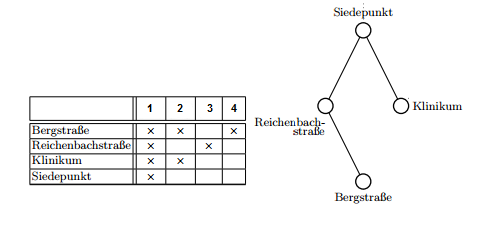
\includegraphics[width=\textwidth]{img/dane.png}
\caption{Dane podstawowe}
\label{dane_podstawowe}
\end{center}
\end{figure}

Na rysunku \ref{dane_podstawowe}\footnote{Dane zaczerpnięto z artykułu: Modeling Preferences over Attribute Sets in
Formal Concept Analysis, Sergei Obiedkov} przedstawiono tabelę z danymi i tabelę relacji w których pozostają klasy dla tych danych. Poniżej znajdują się szczegółowe wyniki dla tego zbioru.\\

Dla tego przypadku tworzone jest następujące mapowanie wartości atrybutów na liczby naturalne:\\

\begin{itemize}
\item 0 i 3 - vegetarian meal
\item 1 i 4 - non-vegetarian meal without pork
\item 2 i 5 - other meal
\item 3 i 7 - meal containing alcohol
\end{itemize}

Atrybuty 4, 5, 6 i 7 powstają w wyniku połączenia dwóch zbiorów.\\

W dalszej częśći tej sekcji dla skrócenia zapisów kandydaci będą opisywani trójką w postaci (0 - (12, 4)), gdzie pierwsza wartość jest indeksem atrybutu, a dwa kolejne to liczniki mówiące o wsparciu w klasach decyzyjnych.

\subsubsection{Relacja ścisła}

W przypadku gdy relacja ma zachodzić w sposób ścisły algorytm znajduje następujące minimalne wzorce kontrastowe:

\begin{enumerate}
\item (other meal) $=>$ (meal containing alcohol) \label{res1}
\item (non-vegetarian meal without pork, meal containing alcohol) $=>$ () \label{res2}
\item (other meal, meal containing alcohol) $=>$ () \label{res3}
\end{enumerate}

Przebieg algorytmu dla tego przypadku, przedstawia się następująco:\\

W pierwszej iteracji algorytm nie odnajduje żadnych wzorców. Kandydaci: (0 - (12, 4)), (4 - (12, 4)), (5 - (8, 0)), (6 - (4, 0)) są odrzucani,
a dalszej analizie podlegają kandydaci: (1 - (5, 3)), (2 - (2, 2)), (7 - (3, 1)), (3 - (3, 1)). Kandydaci 0 i 4 są odrzucani ponieważ zbiór pusty jest ich generatorem, a kandydaci 5 i 6 ponieważ relacja nie jest dla nich spełniona ani razu.\\

W drugiej iteracji algorytm znajduje minimalne wzorce (2, 7 - (0, 1)) mapowany na \ref{res1}, (1, 3 - (0, 0)) \ref{res2} oraz (2, 3 - (0, 0)) \ref{res3} do analizy pozostaje 1 kandydat (1, 7 - (1, 1)) z którego nie można już wygenerować kandydatów 3 elementowych, a kandydaci (1, 2 - (2, 2)) i (3, 7 - (1, 0)) są odrzucani.\\

W przypadku gdy nie wykorzystuje się własności związanej z generatorami, przebieg algorytmu wygląda następująco:\\

W pierwszej iteracji tylko dwóch kandydatów jest wykluczanych z dalszej analizy: (5 - (8, 0)), (6 - (4, 0)). W związku z tym w drugim kroku jest generowanych więcej kandydatów z których aż 11 podlega dalszej analizie: (0, 1 - (5, 3)), (0, 2 - (2, 2)), (0, 4 - (12, 4)), (1, 2 - (2, 2)), (1, 4 - (5, 3)), (2, 4 - (2, 2)), (0, 7 - (3, 1)), (1, 7 - (1, 1)), (4, 7 - (3, 1)), (0, 3 - (3, 1)), (3, 4 - (3, 1)). W kolejnym kroku 8 kandydatów o 3 elementach zostaje do dalszej analizy i dalej 2 kandydatów 4 elementowych.

\subsubsection{Relacja nieścisła}

W przypadku gdy relacja ma zachodzić w sposób nie ścisły algorytm znajduje następujące minimalne wzorce kontrastowe:

\begin{enumerate}
\item (other meal) $=>$ (other meal)
\item (other meal) $=>$ (meal containing alcohol)
\item (meal containing alcohol) $=>$ (meal containing alcohol)
\item (non-vegetarian meal without pork, meal containing alcohol) $=>$ ()
\item (other meal, meal containing alcohol) $=>$ ()
\item () $=>$ (non-vegetarian meal without pork, meal containing alcohol)
\item () $=>$ (other meal, meal containing alcohol)
\end{enumerate}

\subsubsection{Równoważność}

W przypadku gdy relacja ma zachodzić w sposób równoważny algorytm znajduje następujące minimalne wzorce kontrastowe:

\begin{enumerate}
\item (other meal) $=>$ (other meal)
\item (meal containing alcohol) $=>$ (meal containing alcohol)
\item (non-vegetarian meal without pork, meal containing alcohol) $=>$ ()
\item (other meal, meal containing alcohol) $=>$ ()
\item () $=>$ (non-vegetarian meal without pork, meal containing alcohol)
\item () $=>$ (other meal, meal containing alcohol)
\end{enumerate}

\subsection{Wyniki dla złożonych danych}

Algorytm został sprawdzony pod względem wydajności na danych pochodzących z repozytorium \textit{UCI}: Car Evaluation Data Set\footnote{http://archive.ics.uci.edu/ml/datasets/Car+Evaluation}.\\

Zbiór jest podzielony na 4 klasy określające akceptowalność samochodu ze względu na: koszt zakupu, koszt utrzymania, liczbę drzwi, liczbę miejsc, pojemność bagażnika i wskaźnik bezpieczeństwa pojazdu.\\

W zbiorze wyróżniono 4 klasy: nieakceptowalny, akceptowalny, dobry i bardzo dobry. Przyjęto, że pomiędzy klasami zachodzi relacja od najgorszej do najlepszej wg wymienionej kolejności. Zbiór zawiera łącznie 1728 obiektów, opisywanych przez 21 unikalnych ze względu na kolumny wartości atrybutów.\\

Obliczenia przeprowadzone dla całego zbioru są więc wykonywane na blisko $3*10^6$ elementów w której każdy obiekt posiada 42 atrybuty. Charakterystyka zbioru jest na tyle niesprzyjająca, że w kolejnych iteracjach bardzo mało wyników jest odrzucanych, poprawnie klasyfikowanych lub uznawanych za generator. Pełne wyniki otrzymane dla omawianego zbioru znajdują się w pliku wyniki.txt. W tabeli poniżej zaprezentowane są wyniki ilościowe dla obliczeń przeprowadzonych dla całego zbioru. Parametry drzewa mieszajacego: pageSize = 100, key = 47. Poszukiwano wzorców dla relacji nieściełej, wykorzystując własność Terleckiego.

\vspace{0.5cm}

\begin{tabular}{|r|r|r|r|r|}
\hline
Długość & Znalezionych & Do analizy & Odrzuconych & Czas iteracji \\ \hline
1  & 2 & 40 & 0 & 00:00:07.967 \\ \hline 
2  & 53 & 727 & 0 & 00:00:55.509 \\ \hline
3  & 4 & 7932 & 4 & 00:03:54.407 \\ \hline
4  & 16 & 57773 & 16 & 00:12:32.015 \\ \hline
5  & 138 & 294890 & 267 & 00:28:11.867 \\ \hline
6  & 358 & 1073453 & 1159 & 00:44:27.682 \\ \hline
7  & 402 & 2767984 & 1897 & 00:58:16.358 \\ \hline
8  & 347 & 4894458 & 2090 & 01:12:06.853 \\ \hline
9  & 210 & 5539918 & 1637 & 01:14:27.725 \\ \hline
10 & 62 & 3489242 & 728 & 00:51:50.042 \\ \hline
11 & 5 & 859068 & 121 & 00:14:57.773 \\ \hline
12 & 0 & 0 & 4 & 00:00:20.830 \\ \hline

\end{tabular}

W tabeli poniżej, dla porównania zaprezentowano wyniki uzyskane w przypadku gdy przy tworzeniu zbiorów kandydujących odrzucane były te zbiory których podzbiór był jednocześnie generatorem i minimalnym wzorcem kontrastowym.

\vspace{0.5cm}

\begin{tabular}{|r|r|r|r|r|}
\hline
Długość & Znalezionych & Do analizy & Odrzuconych & Czas iteracji\\ \hline
1 & 2 & 40 & 0 &  00:00:08.637 \\ \hline 
2 & 53 & 727 & 0 & 00:01:04.399 \\ \hline
3 & 4 & 7936 & 0 & 00:04:27.911 \\ \hline
4 & 16 & 57900 & 8 & 00:13:41.542 \\ \hline
5 & 138 & 296827 & 89 & 00:31:31.924 \\ \hline
6 & 358 & 1091632 & 319 & 00:49:20.457 \\ \hline
7 & 402 & 2878263 & 529 & 01:00:49.850 \\ \hline
8 & 347 & 5322277 & 541 & 01:16:16.170 \\ \hline
9 & 210 & 6555566 & 490 & 01:29:21.114 \\ \hline
10 & 62 & 4826364 & 305 & 01:10:39.947 \\ \hline
11 & 5 & 1604811 & 82 & 00:26:38.900 \\ \hline
12 & 0 & 0 & 5 & 00:00:45.475 \\ \hline
\end{tabular}

\vspace{0.5cm}

Zawrtość tabeli należy interpretować w następujący sposób: kandydaci o długości 3 zostali wygenerowani w czasie 120ms, wygenerowano łącznie 7900 takich kandydatów, z czego 4 zostały uznane za minimalne wzorce. Analiza kandydatów długości 3 trwała 4 minuty 27 sekund. Obliczenia przeprowadzono na komputerze z procesorem Intel i7 3.4GHz, 16GB ram.\\

Uzyskane czasy wydają się być akceptowalne. Łącznie znaleziono 1597 wzorców.\\

\subsubsection{Zużycie pamięci}

Na wykresie \ref{pamiec} przedstawiono zależność zużycia pamięci w czasie. Pomiary zostały wykonywane z wykorzystaniem mechanizmów GC i próbkowania w 3 sekundowych odstępach czasu.

\begin{figure}[h!]
\begin{center}
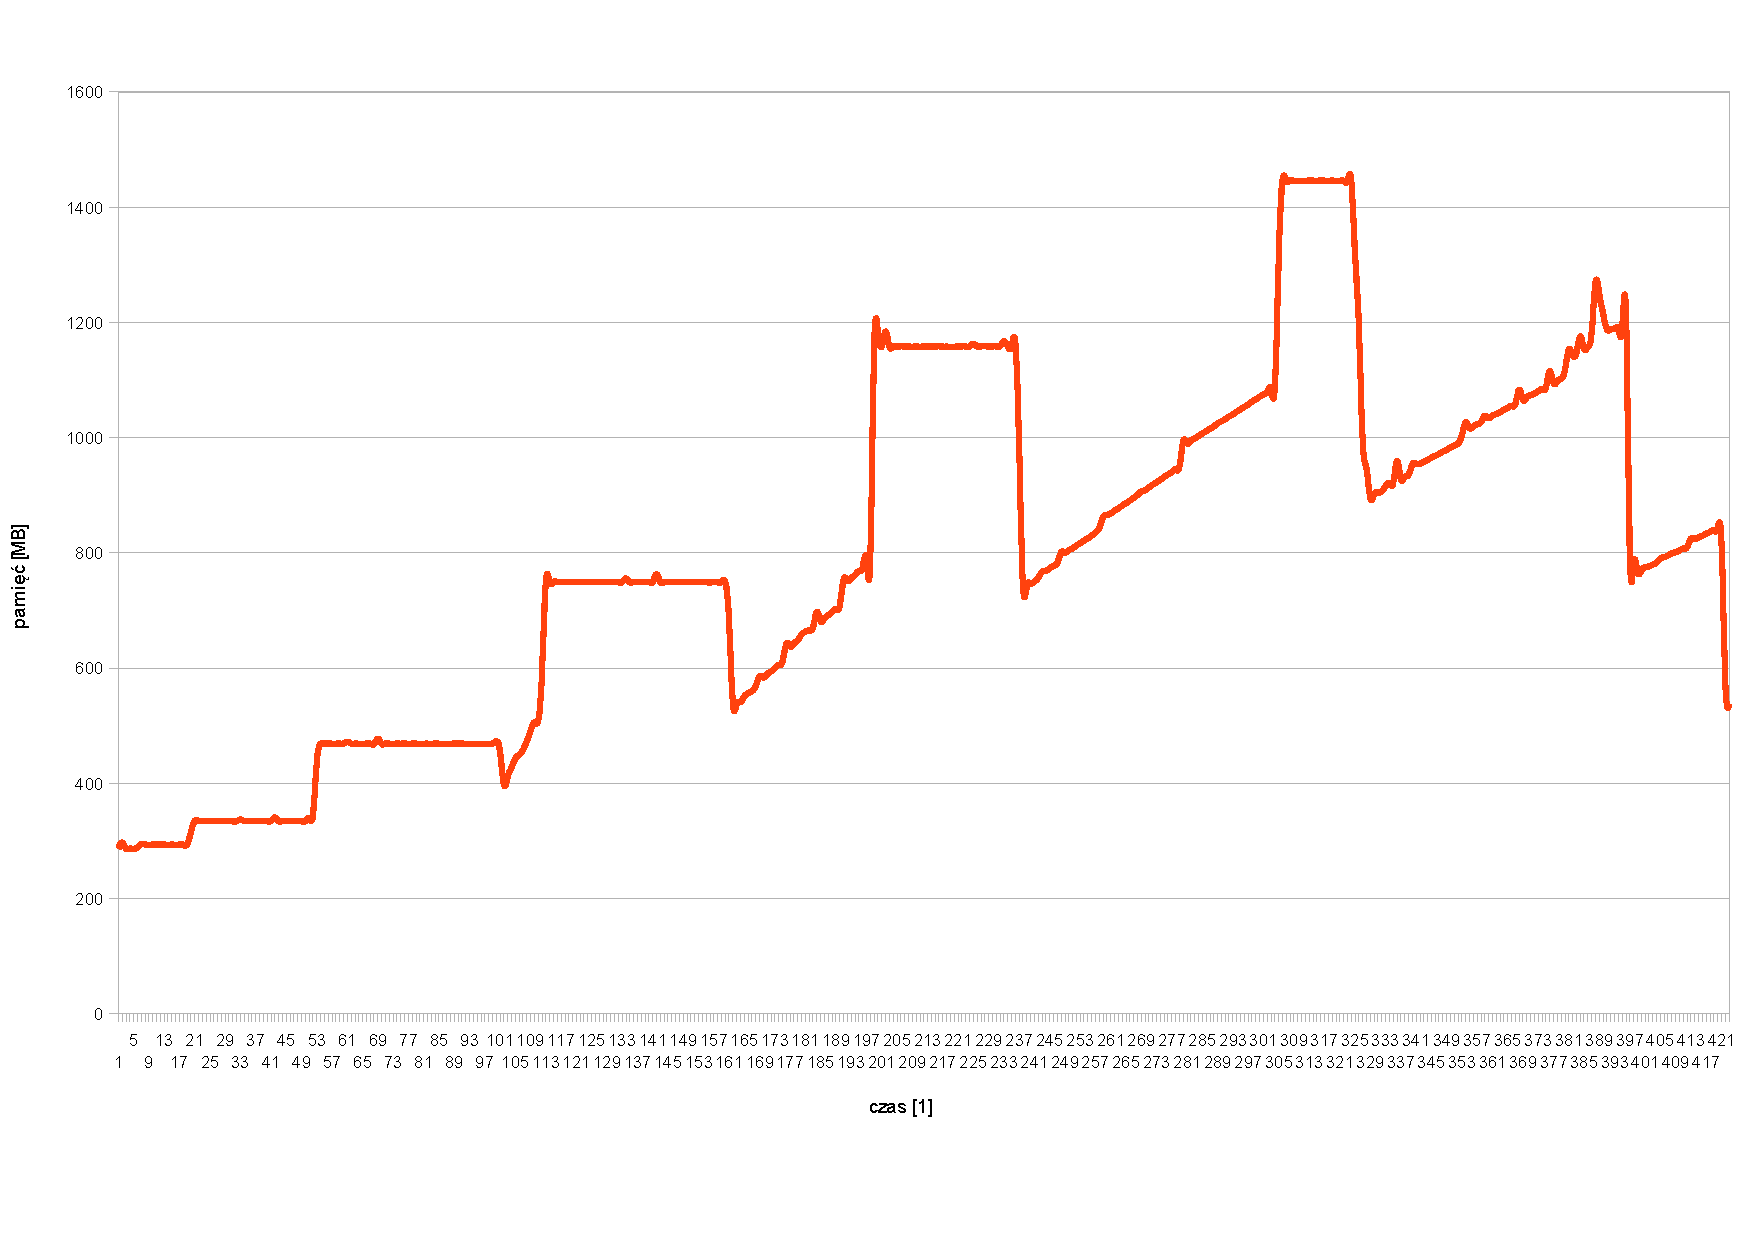
\includegraphics[width=\textwidth]{img/pamiec.pdf}
\caption{Wykres wykorzystania pamięci w czasie dla zbioru cars}
\label{pamiec}
\end{center}
\end{figure}

\section{Wnioski}

\begin{enumerate}

\item Mimo, że w implementacji algorytmu dominującą operacją jest wyszukiwanie wspieranych przez transakcję kandydatów, okazuje się, że również generowanie kolejnej generacji kandydatów jest kosztowne obliczeniowo i należy poświęcić uwagę, na możliwie wydajne zaimplementowanie tego fragmentu kodu. 

\item Wydaje się, że w algorytmie warto było by dodać parametr związany z minimalnym wsparciem, który pozwoliłby na odrzucanie większej ilości zbiorów kandydujących. Z praktycznego punktu widzenia, mając na uwadze fakt, że zbiór w którym wyszukiwane są wzorce ma liczność równą kwadratowi zbioru wyjściowego reguły o bardzo małych wsparciach, mogą nie mieć praktycznego znaczenia.

\item W czasie wielogodzinnego testu algorytm pracował stabilnie, chociaż można przypuszczać, że dla danych o dużej ilości cech (np. kilkaset) konieczne było by przechowywanie kandydatów w pamięci trwałej.

\end{enumerate}

\section{Podział zadań}

\begin{itemize}
\item Bartosz Górski - implementacja przetwarzania danych wejściowych, opis zadania
\item Marcin Kaczyński - implementacja ogólnej architektury, implementacja algorytmu, prace nad optymalizacją, implementacja interfejsów dla użytkownika, przygotowanie wyników, opis szczegółów implementacji i wyników działania algorytmu
\item Paweł Sokołowski - implementacja drzewa mieszającego, prace nad optymalizacją, przygotowanie wyników, opis drzewa mieszającego i badanie wydajności drzewa, opisy złożoności, opis danych
\end{itemize}

\appendix
\section{Podręcznik użytkownika}

Do uruchomienia aplikacji wymagany jest zainstalowany .NET Framework 4.0. Nie jest konieczna instalacja dodatkowych programów, bibliotek lub komponentów. Aplikacja została przygotowana w dwóch wersjach: x86 oraz x64, dla dużych zbiorów danych zaleca się korzystanie z wersji x64.\\

Aplikacja posiada prosty interfejs konsolowy. Uruchomienie sprowadza się do wykonia komendy \textit{UniversalPreferences parametry}, gdzie parametry należy podać w formacie klucz:wartosc:

\begin{itemize}
\item data:sciezka - ścieżka do pliku z danymi
\item relations:sciezka - ścieżka do pliku z relacjami
\item delim:znak - znak dzielący kolumny w pliku danych
\item index:numer - indeks kolumny z danymi
\item pageSize:liczba - rozmiar strony w drzewie mieszającym
\item key:liczba - klucz mieszający
\item relationType:wartosc - {NonStrict, Strict, Equals}
\item method:T - {T - metoda Terleckiego, G - wykorzystanie generatorów, P - wersja podstawowa}
\end{itemize}

Parametry można podawać w dowolnej kolejności. Ostatnie 3 parametry są opcjonalne - ich domyślne wartości to: pageSize = 100, key = 47, relationType = NonStrict. Spacje w nazwach plików nie są dopuszczalne.\\

Aby zapisać wyniki zwracane przez program, należy przekierować standardowe wyjście na plik docelowy.\\

Przykładowe wykonanie może wyglądać następująco:\\

UniversalPreferences data:cardata.txt relations:relation.txt index:6 delim:,


\bibliographystyle{plain}
\bibliography{bibliografia}

\end{document}
